
\documentclass[11pt]{article}

\usepackage[final]{acl}
\usepackage{times}
\usepackage{latexsym}
\usepackage[T1]{fontenc}
\usepackage[utf8]{inputenc}
\usepackage{microtype}
\microtypesetup{stretch=25,shrink=35}
\usepackage{inconsolata}
\usepackage{graphicx}
\usepackage{booktabs}
\usepackage{xurl}   % break long URLs at any character (fixes bib overfull)
\usepackage{enumitem}
\usepackage[normalem]{ulem}   % \uline: underline that breaks across lines

% Let a tall double-column float sit at the top of a text page, so Table 1
% stays inside the 5-page main content rather than deferring past it.
\renewcommand{\dbltopfraction}{0.9}
\renewcommand{\dblfloatpagefraction}{0.7}
\setcounter{dbltopnumber}{3}

% Align floats to the top (not vertical center) on float-only pages.
\makeatletter
\setlength{\@fptop}{0pt}
\makeatother

% Tighten float/caption separation to fit the content within the page limit.
\setlength{\abovecaptionskip}{4pt}
\setlength{\belowcaptionskip}{0pt}
\setlength{\textfloatsep}{9pt plus 2pt minus 2pt}
\setlength{\floatsep}{10pt plus 2pt minus 2pt}
\setlength{\intextsep}{10pt plus 2pt minus 2pt}

\title{From Full Game State to Live Commentary: A Data-to-Text Pipeline and Corpus for \textit{Age of Empires II}}

\author{
  Siewart van Wingerden\textsuperscript{1} \quad
  Mari\"et Theune\textsuperscript{2} \quad
  Lorenzo Gatti\textsuperscript{2} \\
  \textsuperscript{1}Studio Platypus \quad
  \textsuperscript{2}Human Media Interaction, University of Twente \\
  \texttt{siewart@studioplatypus.nl} \quad
  \texttt{\{m.theune,l.gatti\}@utwente.nl}
}

\begin{document}
\maketitle

\begin{abstract}
  We present SAGE (Semantic Abstraction \& Generation from Events), a modular data-to-text pipeline that converts continuous \textit{Age of Empires II} (AoE2) game-state snapshots and events into live text commentary updates, pairing rule-based content selection with a large language model (LLM) realizer. Its content selection operationalizes how human commentators forage the game for information through two independently ablatable strategies: \emph{Expert Insights} (strategic context) and \emph{Event Structuring} (grouping parallel events). Alongside the pipeline we release its underlying corpus: continuous full game-state snapshots for $3{,}100$ ladder and $176$ tournament AoE2 matches ($142$ with paired professional commentary video), to our knowledge the first full-state corpus for a complex esports title. We also report on a preliminary user study with $33$ AoE2 viewers.
\end{abstract}

\section{Introduction}
Watching esports (competitively played video games) is a mainstream spectator activity, and much of its appeal comes from commentators who narrate, contextualize, and dramatize a match in real time \citep{kempecook2019,li2020}. High-quality live commentary is resource-intensive and concentrated at top tournaments, leaving most competitive matches (and players reviewing them) without narrative guidance. Because the game engine mediates every player action, the full match state is available as data, making automated commentary an attractive data-to-text (D2T) application.

We address three gaps. First, the human elements are often overlooked: few systems model the strategies commentators use to select relevant state for their audience, and engagement is rarely validated with the target audience; instead, reference-based overlap metrics are used. The rare human evaluation is of limited scope and, while raters understand the game, esports viewership is never reported \citep{ishigaki2023,wang2024,elarewaju2020}. Second, most esports-commentary systems consume sparse event logs or limited metadata, or target games with a limited state space. For instance, \citet{wang2024} generate commentary from ten high-level event types. Third, datasets available for NLG research generally also focus on these sparse logs or games with limited state complexity, and rarely include paired commentary video; each covers one of these aspects rather than combining them \citep{wang2024,ishigaki2021,zhang2024}.

We address all three: SAGE turns continuous AoE2 game-state snapshots into minute-by-minute text updates (online sports commentary) \citep{pavzanin2022,lewandowski2012}. We contribute \textit{a hybrid D2T pipeline} that abstracts a dense, parallel event stream into reportable events, enriches them from state snapshots and a knowledge base, and realizes text with an LLM, using two independently ablatable engagement modules based on commentator strategies (Section~\ref{sec:pipeline}); the \textit{game-state dataset} consisting of $176$ tournament matches, $142$ with paired professional commentary video and an extra $3{,}100$ recent ladder matches (Section~\ref{sec:corpus}); and \textit{a preliminary user study} ($N=33$ target-audience spectators) testing each module's effect on engagement and linguistic quality (Section~\ref{sec:study}).

\section{Related Work}
\paragraph{Esports and game commentary}
Early esports-focused systems generated narratives from game logs (e.g., Bardic \citep{barot2017}) or grammar-based recaps trained on esports commentator transcripts \citep{elarewaju2020}. Closest to our setting, \citet{wang2021, wang2024, wang2025} generate commentary from event records with neural and LLM realizers, but report reduced control over content selection and only limited viewer evaluation. \citet{zhang2022} compare rule-based and LLM realization; \citet{zhang2024} pair events with commentator audio and chat in a multimodal dataset; and \citet{kim2025} compress match data into LLM-friendly summaries. All of this work targets DotA2 or League of Legends. These are Multiplayer Online Battle Arena (MOBA) games where each player controls one hero and the state and event spaces are far smaller than AoE2's. One genre exception is racing games, which pair video with limited state data \citep{ishigaki2021}, but again with a narrow event space. For other sports, data-to-text covers simulated \citep{voelz1998} and real \citep{taniguchi2019} soccer and post-hoc match reports \citep{vanderlee2017}.

\paragraph{Data-to-text pipelines}
Modular pipelines are often compared with (statistical) end-to-end systems as trading fluency for control \citep{gatt2018}. \citet{castroferreira2019} found that a pipeline produced better text than end-to-end generation. Recently, LLMs and new deployment methods such as multi-agent end-to-end systems score better on automatic metrics and semantic adequacy \citep{osuji2024,osuji2025}. Surveying neural D2T, \citet{lin2024} list limited controllability among remaining challenges and conclude that ``introducing a content planning stage before text generation can effectively enhance controllability and faithfulness''. For game commentary, \citet{zhang2022} find that ``fusing'' a rule-based generator with a neural one best balances accuracy and fluency.

\paragraph{Corpora}
Public esports resources most often cover sparse event logs or compact-state games: League of Legends replay packets \citep{zhu2025}, and player trajectories in ESTA \citep{xenopoulos2022} for a first-person shooter, in which each player controls a single character. Within the same genre as AoE2 we find the SC2EGSet for StarCraft~II \citep{bialecki2023} and AoE2 event logs \citep{liss2024}. Most are not aimed at NLG or need heavy pre-processing, and several are hard to obtain: the multimodal Game-MUG \citep{zhang2024} is event-level and not openly released, and \citet{wang2024} ship tools to regenerate their data rather than the data itself. \citet{ishigaki2021} provide a racing-game commentary dataset pairing video with structured telemetry, but limited to Japanese and a narrow state space.

\section{The SAGE Pipeline}
\label{sec:pipeline}
\textbf{Age of Empires II} (Figure~\ref{fig:captureage}) is a real-time strategy game in which opposing players, each representing one of many \emph{civilizations} with different bonuses, simultaneously gather resources, grow an economy of worker units (\emph{villagers}), advance through four \emph{Ages} that unlock stronger units and technologies, and build armies to disrupt each other's economy and claim victory. The map is procedurally generated and partly hidden by a \emph{fog of war}, so players must scout and adapt. Our pipeline must therefore handle economic and military actions unfolding in parallel.

\begin{figure}[t]
  \centering
  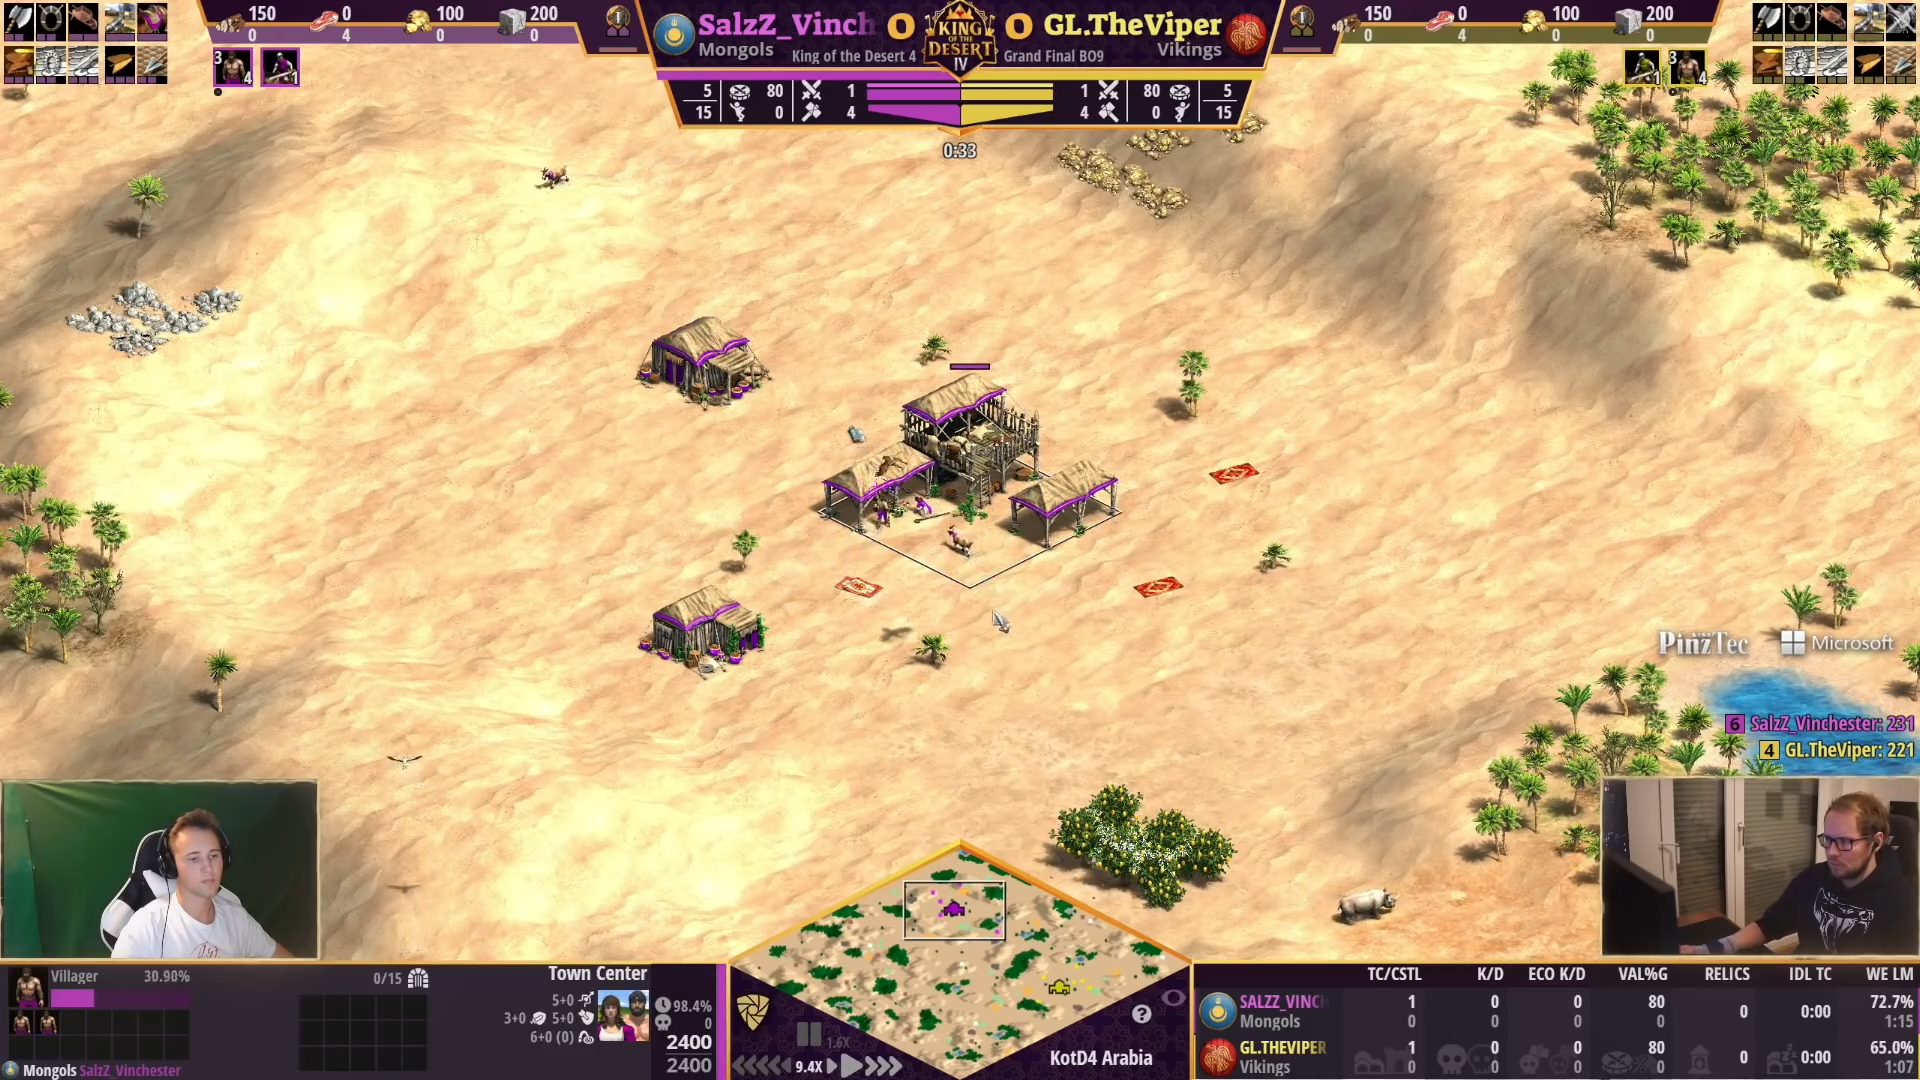
\includegraphics[width=\linewidth]{aoe2-esports-screenshot.png}
  \caption{\emph{Age of Empires II} as shown in \emph{CaptureAge} during a King of the Desert~IV match. CaptureAge creates a live re-rendering from game-state data and low-level events, which SAGE turns into commentary.}
  \label{fig:captureage}
\end{figure}

\begin{figure}[t]
  \centering
  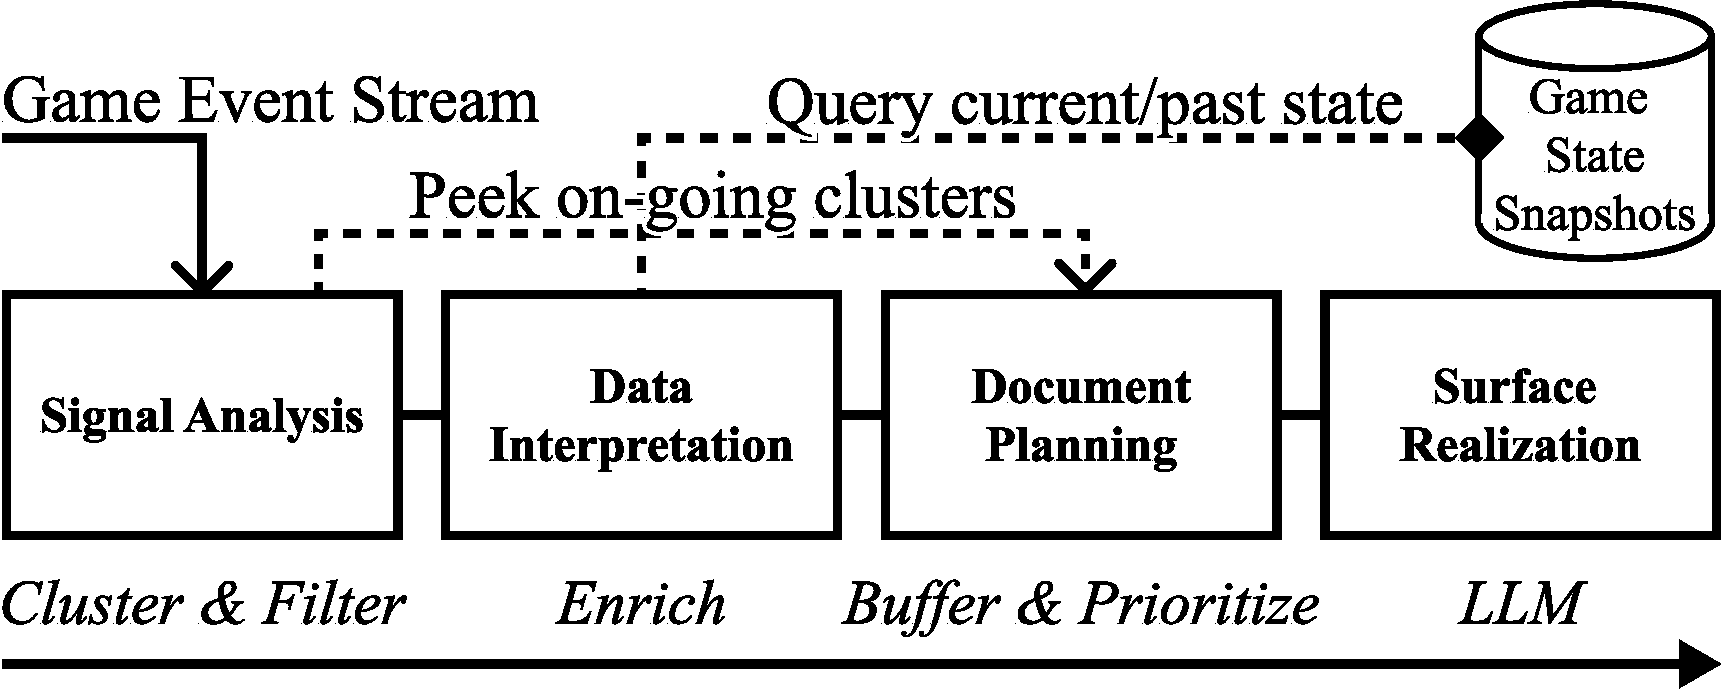
\includegraphics[width=0.82\linewidth]{pipeline-v2.pdf}
  \caption{The SAGE pipeline parses a symbolic event stream and game-state snapshots into realized text.}
  \label{fig:pipeline}
\end{figure}

\subsection{Architecture}
SAGE follows the four-stage architecture of \citet{reiter2007} (Figure~\ref{fig:pipeline}). Data arrives incrementally and the system plans and realizes without knowledge of future events, so it runs as if in a live setting, and could be integrated into a live application.

\paragraph{Signal analysis}
The raw input is a symbolic event stream and periodic full world-state snapshots. An \emph{event} here is emitted from a discrete call the game engine makes while applying its own rules and executing player commands (e.g., a unit taking damage or dying, or a building or technology starting and completing). SAGE pairs them with snapshots windowed at $60$\,s. We preprocess events in two ways. Damage and death events are clustered into battles with ST-DBSCAN \citep{birant2007}, a density-based clustering method with a temporal distance. It attributes two events to the same battle when they lie within $\varepsilon$ map tiles \emph{and} $\tau$ seconds of one another and their neighborhood holds at least \texttt{minPts} events ($\varepsilon=14$ tiles, $\tau=60$\,s, $\texttt{minPts}=10$). This method supports a dynamic number of simultaneous battles, which range from a small skirmish to a full engagement along shifting frontlines. Because the input arrives in chronological order, a cluster can be closed and released once $\tau$ seconds pass, enabling live reporting of resolved or stalled battles. Downstream stages can also read an open cluster, or force it closed, to report an ongoing fight. Other event types, such as constructions (Castles, Town Centers, Towers), are kept by filtering on building type and location.

\paragraph{Data interpretation}
Clustered events are enriched from the snapshot current at event time (or an earlier cached one), simulating live operation. Enrichment follows the Actuator--Environment--Performance+Sensors (A--E--P+S) scheme \citep{russell1995, dodge2018}, reflecting how commentators forage for information \citep{dodge2018,penney2021,VanWingerden2026}: the \emph{Actuator} is the event; the \emph{Environment} is the state it occurs in (location, battle participants); \emph{Performance} is who leads on key metrics (e.g., economy); and \emph{Sensors} capture what each side can currently see. To help readers visualize the game map, we add narrative location anchors (names for regions and landmarks) using cardinal and relative directions, so an event at numerical map coordinates is reported at ``Blue's forward gold mine''.

Enrichment adds and updates the pipeline's data, and text is generated only during realization; however, in the following example we show the steps as text. We start from the Actuator, \emph{``Red's three scouts kill a Villager''}, derived from a battle event cluster. Environment and Performance give \emph{``\uline{With Forging now in}, Red's three scouts kill a Villager. \uline{Red is now three Villagers ahead}''}, adding information from the game state snapshots; the location anchors and the game clock give \emph{``\uline{16:32 ---} \ldots\ \uline{on the forward woodline}''}.

\paragraph{Planning and realization}
The planner opens with two introductions: the players and civilizations, and the game map. It buffers enriched events and flushes them when a pending battle's cooldown expires, or at game end. Each content unit is realized by Gemini~2.5~Flash, chosen for low first-token latency, at temperature~1 with a fixed seed. All previously realized text is given as prior turns so references and tone are consistent. Its prompt has three parts: a fixed system instruction, a communicative goal, and the preprocessed JSON with numerical identifiers replaced by names and human-friendly timestamps. Writing style instructions (simple present, copula deletion, spatiotemporal anchoring \citep{lewandowski2012}, matching the live-update register) are added to ensure consistency. A module's prompts are added only when that module is enabled, so the final combined prompt changes with the module configuration.
The state selected in the previous stages and additional state facts are added for grounding, and we discourage unsupported claims through negative prompting. See Appendix~\ref{app:prompts} for an overview.

Realization, with the register effects underlined, turns the data of our earlier example into \emph{``16:32 --- With Forging now in, Red's three scouts \uline{waste no time --- they spot a Villager} on the forward woodline! Red \uline{surges ahead with} a three-Villager advantage.''}

\subsection{Engagement Modules}
\label{sec:modules}
Engagement strategies are ablatable modules that add steps to any pipeline stage and can be enabled independently. The two strategies below, and the event and context types the pipeline surfaces, were informed by two preparatory studies \citep{VanWingerden2026}. In the first, building on analyses of a game in the same genre \citep{dodge2018,penney2021}, we coded a professional AoE2 co-cast (two commentators with complementary roles, \citealp{kempecook2019}) for both information source (e.g., descriptive game state or expert domain knowledge) and communicative intent, and two further co-casts for intent alone. This informed our use of the A--E--P+S format found by \citet{dodge2018}, but also highlighted the need for information outside the game state. Utterances describing what is happening are mostly derived from observations of the game state ($78\%$, $n=86$). But reasoning about the state relies more on external knowledge sources: domain knowledge and analytical inference together cover $86\%$ of strategy discussion ($n=38$) and $77\%$ of strategy prediction ($n=34$). In the second study, a formative survey, $57$ AoE2 viewers watched a manually created video summary and rated how relevant different event types were for understanding the match. \textit{Battles that cost economic units} was the highest-rated content. In open answers viewers said they would also have liked to see the missing economic consequences and causal links of those events.

\begin{itemize}[noitemsep,topsep=2pt,leftmargin=*]
  \item \textbf{Expert Insights} adds the domain knowledge and analytical inference not contained in the game state. Strategic civilization information comes from the AoE2 Fandom wiki and player trivia from Liquipedia,\footnote{\url{https://ageofempires.fandom.com/}, \url{https://liquipedia.net/ageofempires/}} compiled offline into a static knowledge base. A fuzzy-logic detector scores unit and building counts and positions, technology state and worker distribution to label high-level strategies (e.g., ``Tower Rush'', ``Fast Castle''), which are added during data interpretation. Its rule templates were drafted by an LLM and manually verified. Additional facts are injected into the realizer prompt with causal explanations (e.g., ``Exposed gold mines are vulnerable to Archers'') so it can place events in context.
  \item \textbf{Event Structuring} focuses on the game's parallelism: unlike traditional sports built around a single ball, several fights and economic decisions happen at the same time. It groups related events during document planning so the realization step can express causal connections. The planner buffers events for at most $180$ game seconds or five events, and groups those overlapping in time. An LLM system prompt is used to select the most important fights and their causal relations. A separate prompt instruction encourages information asymmetry, which \citet{cheung2011starcraft} identify as a driver of engagement in StarCraft shoutcasting: the realizer contrasts what each side can see with the all-knowing viewer's perspective to create suspense.
\end{itemize}

\section{The Corpus}
\label{sec:corpus}
We release an extended version of the corpus used in the pipeline, to our knowledge the first full game-state set aimed at NLG for a complex esports title. It comprises the \emph{May~2026} set ($3{,}100$ anonymized ranked one-versus-one (1v1) ladder matches from the top~$1{,}000$ players by matchmaking rating) and the \emph{King of the Desert~IV} (KotD~IV) set ($176$ tournament matches, $142$ with commentary video), totaling roughly $120{,}000$ minutes of play and $16$\,M issued player commands (Table~\ref{tab:corpus}). Each match is exported at both $1$\,s and $60$\,s snapshot resolution as columnar tables (Table~\ref{tab:schema}); Appendix~\ref{app:corpus-stats} describes the contents. The windowed tables track every \emph{entity}, meaning every unit and building on the map, alongside each player's economy, technology and visibility. The events we export from the engine were selected based on the preferences reported in the preparatory viewer survey. The state was extracted with CaptureAge, a match-analysis tool that reconstructs a full match and its advanced statistics from a replay or a running game instance.
This corpus enables research on large state spaces, event streams and data frames describing a complex environment in which frequent commands are issued. For $142$ matches it pairs these with professional commentary video narrating the most important events, and with the CaptureAge replay for visual inspection. A full snapshot exceeds what a language model can ingest in real time, so a system must select when and what data to use.

\section{Preliminary User Study}
\label{sec:study}
To investigate the relative contributions of \emph{Expert Insights} and \emph{Event Structuring} to viewer engagement and linguistic quality, we performed a preliminary within-subjects user study using pre-generated texts in the live-update register.

\begin{table*}[t]
  \centering\small
  \setlength{\tabcolsep}{3.5pt}
  \renewcommand{\arraystretch}{0.95}
  \begin{tabular}{@{}l r c r c r r c r r r@{}}
    \toprule
                         & \multicolumn{2}{c}{\textbf{Grand mean}}
                         & \multicolumn{3}{c}{\textbf{Expert Insights}}
                         & \multicolumn{3}{c}{\textbf{Event Structuring}}
                         & \multicolumn{2}{c}{\textbf{Model} $R^2$} \\
    \cmidrule(lr){2-3}\cmidrule(lr){4-6}\cmidrule(lr){7-9}\cmidrule(l){10-11}
    \textbf{Outcome}     & $M$  & 95\% CI      & $\beta$         & 95\% CI          & $p$           & $\beta$      & 95\% CI       & $p$           & marg. & cond. \\
    \midrule
    \multicolumn{11}{@{}l}{\emph{Engageability (MSES motivations)}} \\
    Competitive Nature   & 3.20 & [2.65, 3.74] & \textbf{.20}    & [.05, .34]       & \textbf{.008} & .05          & [$-$.10, .19] & .522          & .02   & .74 \\
    Skill Improvement    & 2.58 & [2.09, 3.08] & \textbf{.19}    & [.07, .30]       & \textbf{.002} & $-$.05       & [$-$.17, .07] & .413          & .02   & .80 \\
    Game Knowledge       & 3.86 & [3.22, 4.51] & .14             & [$-$.03, .32]    & .109          & .02          & [$-$.16, .19] & .854          & .01   & .73 \\
    Skill Appreciation   & 2.53 & [2.08, 2.99] & .10             & [$-$.01, .22]    & .082          & $-$.04       & [$-$.15, .07] & .483          & .02   & .75 \\
    Entertaining Nature  & 2.88 & [2.37, 3.38] & .11             & [$-$.03, .25]    & .124          & .11          & [$-$.03, .25] & .132          & .02   & .71 \\
    Dramatic Nature      & 2.65 & [2.14, 3.17] & .10             & [$-$.05, .25]    & .176          & .01          & [$-$.14, .16] & .856          & .01   & .67 \\
    Vicarious Sensation  & 2.79 & [2.30, 3.29] & \textbf{.25}    & [.10, .40]       & \textbf{.001} & .10          & [$-$.05, .25] & .206          & .03   & .67 \\
    \addlinespace[2pt]
    \multicolumn{11}{@{}l}{\emph{Linguistic quality and comprehension}} \\
    Overall Quality      & 3.82 & [3.41, 4.23] & .08             & [$-$.13, .29]    & .444          & .08          & [$-$.13, .28] & .461          & .02   & .42 \\
    Word Choice          & 4.28 & [3.90, 4.66] & .01             & [$-$.20, .22]    & .905          & .15          & [$-$.06, .35] & .166          & .03   & .38 \\
    Readability          & 4.62 & [4.04, 5.20] & $-$.04          & [$-$.26, .17]    & .685          & $-$.10       & [$-$.31, .12] & .371          & .01   & .43 \\
    Logicality           & 5.61 & [5.28, 5.93] & .04             & [$-$.13, .21]    & .656          & \textbf{.22} & [.05, .39]    & \textbf{.013} & .06   & .34 \\
    Detail Level         & 4.41 & [3.77, 5.05] & \textbf{$-$.24} & [$-$.45, $-$.04] & \textbf{.022} & .06          & [$-$.14, .27] & .538          & .02   & .51 \\
    Reading Thoroughness & 4.56 & [3.77, 5.35] & $-$.15          & [$-$.38, .08]    & .202          & .14          & [$-$.09, .38] & .218          & .02   & .39 \\
    Understanding        & 4.46 & [3.91, 5.02] & .16             & [$-$.04, .36]    & .114          & $-$.12       & [$-$.32, .07] & .217          & .02   & .56 \\
    \bottomrule
  \end{tabular}
  \caption{Study results ($N=33$, $132$ ratings), one linear mixed model per outcome, sum contrasts. The intercept is the grand mean over all four configurations on a 7-point scale and each $\beta$ the deviation from it when that module is on. $R^2$ is Nakagawa's marginal (fixed effects alone) and conditional (fixed and random). Bold is $p<.05$. No interaction between modules was significant; \emph{Detail Level} has a centered neutral 1 = far too much to 7 = far too little.}
  \label{tab:study}
\end{table*}

\paragraph{Stimuli and design}
We generated static commentary using all four configurations (neither module, \emph{Expert Insights}, \emph{Event Structuring}, both) for four KotD~IV matches, giving $16$ texts of roughly $500$--$800$ words. The texts were used as generated, so they still contain realization artifacts such as repetitions, tense slips and occasional attribution errors. In a Latin-square-style design each participant read four texts, seeing every match and configuration once in randomized order, for $132$ evaluated texts.

\paragraph{Participants}
Our participants are active spectators of competitive AoE2 ($32$ of $33$ watch at least weekly), with a well-above-average self-reported skill rating when playing ($M=1600$ Elo, $n=30$), recruited on the AoE2 subreddit in August 2025.

\paragraph{Measures and analysis}
After each text, participants rated seven engageability motivations (adapted from MSES \citep{qian2020}, two items each), five linguistic-quality \citep{callaway2002} and two comprehension items, all on 7-point scales. Per outcome we fitted a linear mixed model with both modules, their interaction and presentation order as fixed effects and random intercepts for match and participant, with sum contrasts, so each coefficient is a deviation from the grand mean. Scale reliability, the model specification, the power analysis and robustness refits are in Appendix~\ref{app:instrument}.

\paragraph{Results}
Engageability was low in absolute terms (Table~\ref{tab:study}): grand means ranged from $2.53$ to $3.86$, well below the neutral midpoint for every motivation but \emph{Game Knowledge} (enjoys using own AoE2 knowledge). Linguistic quality was higher (\emph{Logicality} (logical order of text) $5.61$, \emph{Readability} (fluency) $4.62$): the texts read as coherent and readable. \emph{Expert Insights} significantly raised the three analytical motivations, \emph{Competitive Nature} (enjoys competition, $\beta=.20$, $p=.008$), \emph{Skill Improvement} (reading improves skill, $\beta=.19$, $p=.002$) and \emph{Vicarious Sensation} (as if playing themselves, $\beta=.25$, $p=.001$), and moved perceived \emph{Detail Level} toward ``just right'' ($\beta=-.24$, $p=.022$). \emph{Event Structuring} improved only \emph{Logicality} ($\beta=.22$, $p=.013$). No module interaction was significant, so the modules act independently. However, main effect sizes were much smaller than participant variance (Appendix~\ref{app:instrument}). In closing questions, $16$ of $33$ believed all four texts were machine-generated ($M=3.3/4$, $SD=0.77$).

\paragraph{Open feedback}
Feedback ($96$ of $132$ evaluations) favored strategic importance and high-level context, and preferred a dry, analytical tone, flagging the live-update register as noise, likely because the updates were presented as a single offline text. Trust was limited: correctly realized events were seen as hallucinated. A game-specific example is a mention of Aztec cavalry, which is normally unobtainable. The system failed to mention the unusual way the player had obtained it, leading a participant to see it as a hallucination. We checked every claim participants flagged as implausible against CaptureAge and the source data; each was a real event.

\section{Discussion and Conclusion}
Even as language models improve, turning dense full game state into live commentary remains an unresolved problem. We focused on a vertical slice: completing a full pipeline from game state to live commentary, designing from a human analysis and ending with a human evaluation. Using strategies similar to those of human commentators \citep{dodge2018,penney2021}, we saw modest but significant gains in engagement and linguistic quality with the real target audience, yet the baseline scores for engagement are low. Strategic context raised the motivations related to understanding the events, and structuring events improved only perceived order. However, AoE2 viewers engaging with the static text used in our study were looking for information, not ``hype''. A first direction is to explore the generation of commentary supported by video, rather than text updates. Better ways to express causal links between events, and the context needed to understand them, are another direction indicated by the target audience. Both directions can be explored with the corpus we release alongside the pipeline.

% Acknowledgments coun't toward the page limit, so we move them above the Limitations
\section*{Acknowledgments}
We thank CaptureAge for the technology, MembTV and DonDinardoni for the KotD~IV matches, and NOVA for the commentary videos.

% Everything after this line is not counted toward the page limit
\section*{Limitations}
Our stimulus was static text read after the match, a modality that does not exist for AoE2 and is thus unfamiliar to viewers, who are instead used to live commentary supported by video. We designed our system with the goal of such live commentary in mind. The additional $142$ paired videos are our route toward this real-time narration. The \emph{Event Structuring} implementation groups events by simple heuristics, leaving room for more sophisticated approaches. We evaluated a single opaque proprietary realizer, limiting both reproducibility and our understanding of the scope of its baseline AoE2 knowledge.

\section*{Ethics Statement}
The user study was approved by the University of Twente EEMCS ethics committee. Participants gave informed consent and could withdraw their data. The professional commentary videos in the corpus are redistributed with the commentators' and tournament organizers' written permission. The \emph{May~2026} ladder set is anonymized, with player-identifying information removed (including: in-game name, chat messages, exact skill rating, match IDs, lobby titles and profile IDs). Tournament participants are public competitors and the matches are widely available as broadcast recordings. We release the dataset to the public domain (CC0), except fields derived directly from game content (game-statistics data and in-game strings), which remain subject to XBOX's terms, as do the CaptureAge and AoE2:DE recordings, in accordance with XBOX's Game Content Usage Rules.

\section*{Supplementary Materials Availability Statement}
The SAGE pipeline source, the full corpus, the study stimuli, and the analysis scripts used to produce Table~\ref{tab:study} and additional analyses are available at \url{https://huggingface.co/datasets/Siewart/sage} (DOI \texttt{10.57967/hf/10202}) for the corpus and \url{https://github.com/Siewart/sage} for the source code and study materials.
% For neural use, we suggest encoding underlying feature values rather than categorical names (e.g., the Britons' Archer range bonus rather than the civilization label, or resource and terrain locations rather than the map name) to avoid overfitting to the corpus's specific maps and civilizations.
\bibliography{custom}

\appendix
% ACL formatting guide: "Letter them in sequence and provide an informative
% title: Appendix A. Title of Appendix". 
\makeatletter
\renewcommand{\@seccntformat}[1]{Appendix~\csname the#1\endcsname.\quad}
\makeatother
\counterwithin{table}{section}
\counterwithin{figure}{section}
\renewcommand{\thetable}{\thesection\arabic{table}}
\renewcommand{\thefigure}{\thesection\arabic{figure}}

\section{Prompt Structure}
\label{app:prompts}
Each realizer call is assembled from three layers of prompt plus the data payload (Table~\ref{tab:prompts}). The base layer is identical in every call; the communicative-goal layer is selected by the type of content unit being realized; the module layer is present only for the modules enabled in that ablation configuration, including a negative prompt that is added when \emph{Expert Insights} is disabled to keep the realizer from supplying strategic knowledge of its own. The full text of every prompt is released with the pipeline.\footnote{\label{fn:repo}\url{https://github.com/Siewart/sage/blob/INLG/packages/sage-core/src/gemini/prompts.ts}}

\begin{table}[h]
  \centering\footnotesize
  \setlength{\tabcolsep}{4pt}
  \begin{tabular}{@{}llp{2.9cm}@{}}
    \toprule
    \textbf{Layer} & \textbf{Content}             & \textbf{Present if} \\
    \midrule
    Base           & Role and constraints           & always \\
    Base           & Output format                  & always \\
    Base           & Output language                & always \\
    Base           & Output length                  & always, variable length \\
    Base           & Writing style                  & always \\
    \addlinespace[2pt]
    Goal           & Match introduction             & match-intro \\
    Goal           & Map introduction               & map-intro \\
    Goal           & Event                          & per event\\
    \addlinespace[2pt]
    Module         & \emph{EI} role and constraints & \emph{EI} on; per config variant \\
    Module         & \emph{EI} negative prompt      & \emph{EI} off \\
    Module         & \emph{ES} role and constraints & \emph{ES} on; per goal variant \\
    \addlinespace[2pt]
    Data           & Enriched JSON                  & always; variable module-specific data \\
    Data           & Previous turns                 & 2nd call onwards \\
    \bottomrule
  \end{tabular}
  \caption{Prompt setup per call, with \emph{EI} for \emph{Expert Insights} and \emph{ES} for \emph{Event Structuring}. Base and data layers are the same for all configurations with variables replaced (such as a target word count); the goal layer varies with the content unit; the module layer varies with the ablation configuration.}
  \label{tab:prompts}
\end{table}

\section{Corpus Contents}
\label{app:corpus-stats}
Table~\ref{tab:corpus} breaks down the size of the corpus. Player and civilization matchup counts indicate variety and data biases; the KotD~IV set is deliberately confined to a single popular map to reduce variability. Table~\ref{tab:schema} lists the per-match tables exported, written as Apache~Arrow IPC (and Parquet) and indexed by a JSON descriptor. We also include the CaptureAge and \emph{Age of Empires~II: Definitive Edition} (AoE2:DE) recordings for reference and validation, per-set unit descriptions, and, for KotD~IV, match-to-video timings. Both sets are exported at $1$\,s and $60$\,s snapshot resolution.
\begin{table}[!htb]
  \centering\footnotesize
  \setlength{\tabcolsep}{4pt}
  \begin{tabular}{@{}lrr@{}}
    \toprule
    \textbf{Metric}       & \textbf{KotD~IV}  & \textbf{May~2026} \\
    \midrule
    Matches (total/video) & 176 / 142         & 3{,}100 \\
    Video: solo / co-cast & 118 / 24          & --- \\
    Game min. (tot/vid)   & 6{,}919 / 5{,}548 & 112{,}713 \\
    Commands issued       & 1.09\,M / 0.88\,M & 15.1\,M \\
    Unique players        & 30                & 888 \\
    Player matchups       & 42                & 2{,}735 \\
    Civs (picked / total) & 31 / 35           & 53 / 53 \\
    Civ matchups          & 121               & 1{,}266 \\
    Maps                  & Arabia (100\%)    & Arabia 70\%, +15 \\
    \bottomrule
  \end{tabular}
  \caption{Corpus statistics for the King of the Desert~IV and May~2026 sets. ``Solo''/``co-cast'' = one/two commentators. \emph{1v1 Random Map} is the standard ladder format. Ranked matchmaking draws from a curated pool of $16$, Arabia accounting for 70\%. The percentage follows from player preferences (they can ban and prefer maps before matchmaking) and closely represents the overall map selection. The civilization totals differ because the game gained civilizations between the two sets.}
  \label{tab:corpus}
\end{table}

\begin{table}[h]
  \centering\footnotesize
  \setlength{\tabcolsep}{3pt}
  \begin{tabular}{@{}llp{3.5cm}@{}}
    \toprule
    \textbf{Table} & \textbf{Kind} & \textbf{Contents} \\
    \midrule
    players        & windowed      & stockpiles, population, Age \\
    entities       & windowed      & every unit and building: owner, position, hit points, action \\
    masters        & windowed      & per-owner statistics of each unit and building type \\
    research       & windowed      & technologies finished, started, queued \\
    world          & windowed      & game clock, market rates \\
    fog-of-war     & windowed      & what each player can see \\
    events         & series        & the engine's event stream \\
    commands       & series        & the actions each player issued \\
    map            & record        & terrain and elevation per tile \\
    settings       & record        & lobby configuration \\
    strings        & dict          & lookup for the name IDs \\
    \bottomrule
  \end{tabular}
  \caption{Per-match data tables. \emph{Windowed} tables are fixed-interval snapshots; \emph{series} are timestamped streams of instants; \emph{record} and \emph{dict} are static. The tables share window, player, entity and string identifier columns, as in a relational database.}
  \label{tab:schema}
\end{table}

\section{Study Questionnaire and Analysis}
\label{app:instrument}

\paragraph{Questionnaire}
Participants first answered background questions; the engageability, quality and comprehension items were then asked after each of the four texts, and closing questions at the end. Every item is rated on a 7-point scale; answers are anonymized and, with the participants' permission, released with the analysis scripts. The exact wording of every item is listed in the repository.\footnote{\url{https://github.com/Siewart/sage/blob/INLG/studies/eval/questionnaire.md}} The composition of each construct from its items is defined in the analysis scripts.

Engageability is measured as constructs of two questions per motivation, adapted from the MSES \citep{qian2020} and reported as averages in Table~\ref{tab:study}:
\begin{itemize}[noitemsep,topsep=2pt,leftmargin=*]
  \item \textbf{Competitive Nature:} The enjoyment of high-level competition and rivalry.
  \item \textbf{Skill Improvement:} Watching to learn new strategies and improve one's own gameplay.
  \item \textbf{Game Knowledge:} Interest driven by a deep understanding of the game's mechanics.
  \item \textbf{Skill Appreciation:} Admiring exceptional skills and unique plays by professionals.
  \item \textbf{Entertaining Nature:} Seeking fun and pleasure from the content.
  \item \textbf{Dramatic Nature:} The appeal of uncertainty, comebacks, and underdog stories.
  \item \textbf{Vicarious Sensation:} The feeling of being ``in the game'' and experiencing it through the player.
\end{itemize}

The linguistic-quality \citep{callaway2002} and comprehension items were asked as follows:
\begin{itemize}[noitemsep,topsep=2pt,leftmargin=*]
  \item \textbf{Overall Quality:} Overall, how would you rate the quality of the text?
  \item \textbf{Word Choice:} How appropriate were the word choices in the match updates?
  \item \textbf{Readability:} How hard was it to read the match updates? (\emph{extremely difficult} to \emph{extremely easy})
  \item \textbf{Logicality:} How often did you feel the live updates were presented out of order? (\emph{always} to \emph{never})
  \item \textbf{Detail Level:} How would you rate the level of detail in the match updates? (\emph{far too much} to \emph{far too little}, so 4 is the target rather than 7)
  \item \textbf{Reading Thoroughness:} How much did you skip or skim in order to get to the parts you found interesting? (reversed in analysis)
  \item \textbf{Understanding:} How well do you understand how the match played out?
\end{itemize}
Except for \emph{Detail Level}, every scale is oriented so that a higher score is better.

\paragraph{Reliability}
Across the seven two-item motivation composites, internal consistency is high to very high: Cronbach's $\alpha$ between $.79$ and $.93$, and the correlation between a motivation's two items from $.66$ to $.87$.

\paragraph{Model}
Per outcome we fitted \textit{Score} $\sim$ \textit{EI} $*$ \textit{ES} $+$ \textit{Order} $+\ (1|\textit{Match}) + (1|\textit{Participant})$, where \textit{EI} and \textit{ES} are the two engagement modules, \textit{Order} is the position of the text in that participant's randomized order, and \textit{Match} and \textit{Participant} are random intercepts. Sum contrasts code modules as $\pm 1$, so the intercept is the grand mean over all four configurations and each $\beta$ is the deviation from it when that module is on. Comparisons against the neutral midpoint of the scale are Wilcoxon signed-rank tests with Holm correction.

\paragraph{Variance explained}
Nakagawa's marginal $R^2$, the part of the variance the modules and order explain by themselves, is between $.008$ and $.062$; the conditional $R^2$, which adds the random effects, is between $.341$ and $.795$. The intraclass correlations agree: a median of $.59$ of the variance lies between participants versus $.01$ between matches. \textit{Order} was significant for \emph{Overall Quality} ($\beta=0.19$, $p=.049$).

\paragraph{Robustness}
A Monte Carlo power analysis ($2{,}000$ simulations, using the variability observed in the formative survey) reached $80\%$ power to detect a $0.5$-point effect at $\alpha=.05$ with nine participants, both module effects being within-subject. While linear mixed models (LMMs) are commonly applied to 7-point Likert scales, we also fitted each model as an ordinal mixed model, and again with \textit{Match} as a fixed rather than a random effect. Both alternatives left the LMM conclusions unchanged.

\end{document}
